\section{Review of Graph Neural Networks}

In this section, we introduce the concepts related to the graph neural network (GNN, for short) and breifly survey typical graph neural networks.
We denote a simple graph $\mathcal{G}$ as $\mathcal{G}=(\mathcal{V}, \mathcal{E})$, where $\mathcal{V}$ and $\mathcal{E}$ are the vertex set and the edge set of $\mathcal{G}$, respectively.
Let $n=|\mathcal{V}|$ and $m=|\mathcal{E}|$ as the number of vertices/edges. 
We use $v_i$ $(0 \leq i < n)$ to denote a vertex and $e_{i,j}=(v_i, v_j)$ to denote the edge pointing from $v_i$ to $v_j$.
The adjacency set of $v_i$ is $\mathcal{N}(v_i)=\{v|(v_i, v) \in \mathcal{E}\}$.
We denote a \emph{vector} with a bold lower case letter like $\boldsymbol{x}$ and a \emph{matri}x with a bold upper case letter like $\boldsymbol{X}$.

\subsection{General Structure of Graph Neural Networks}

As illustracted in \figurename~\ref{fig:general_structure_of_gnn}, a typical GNN can be decomposed into three parts: an input layer + several GNN layers + a prediction layer.

\begin{figure}
	\centering
	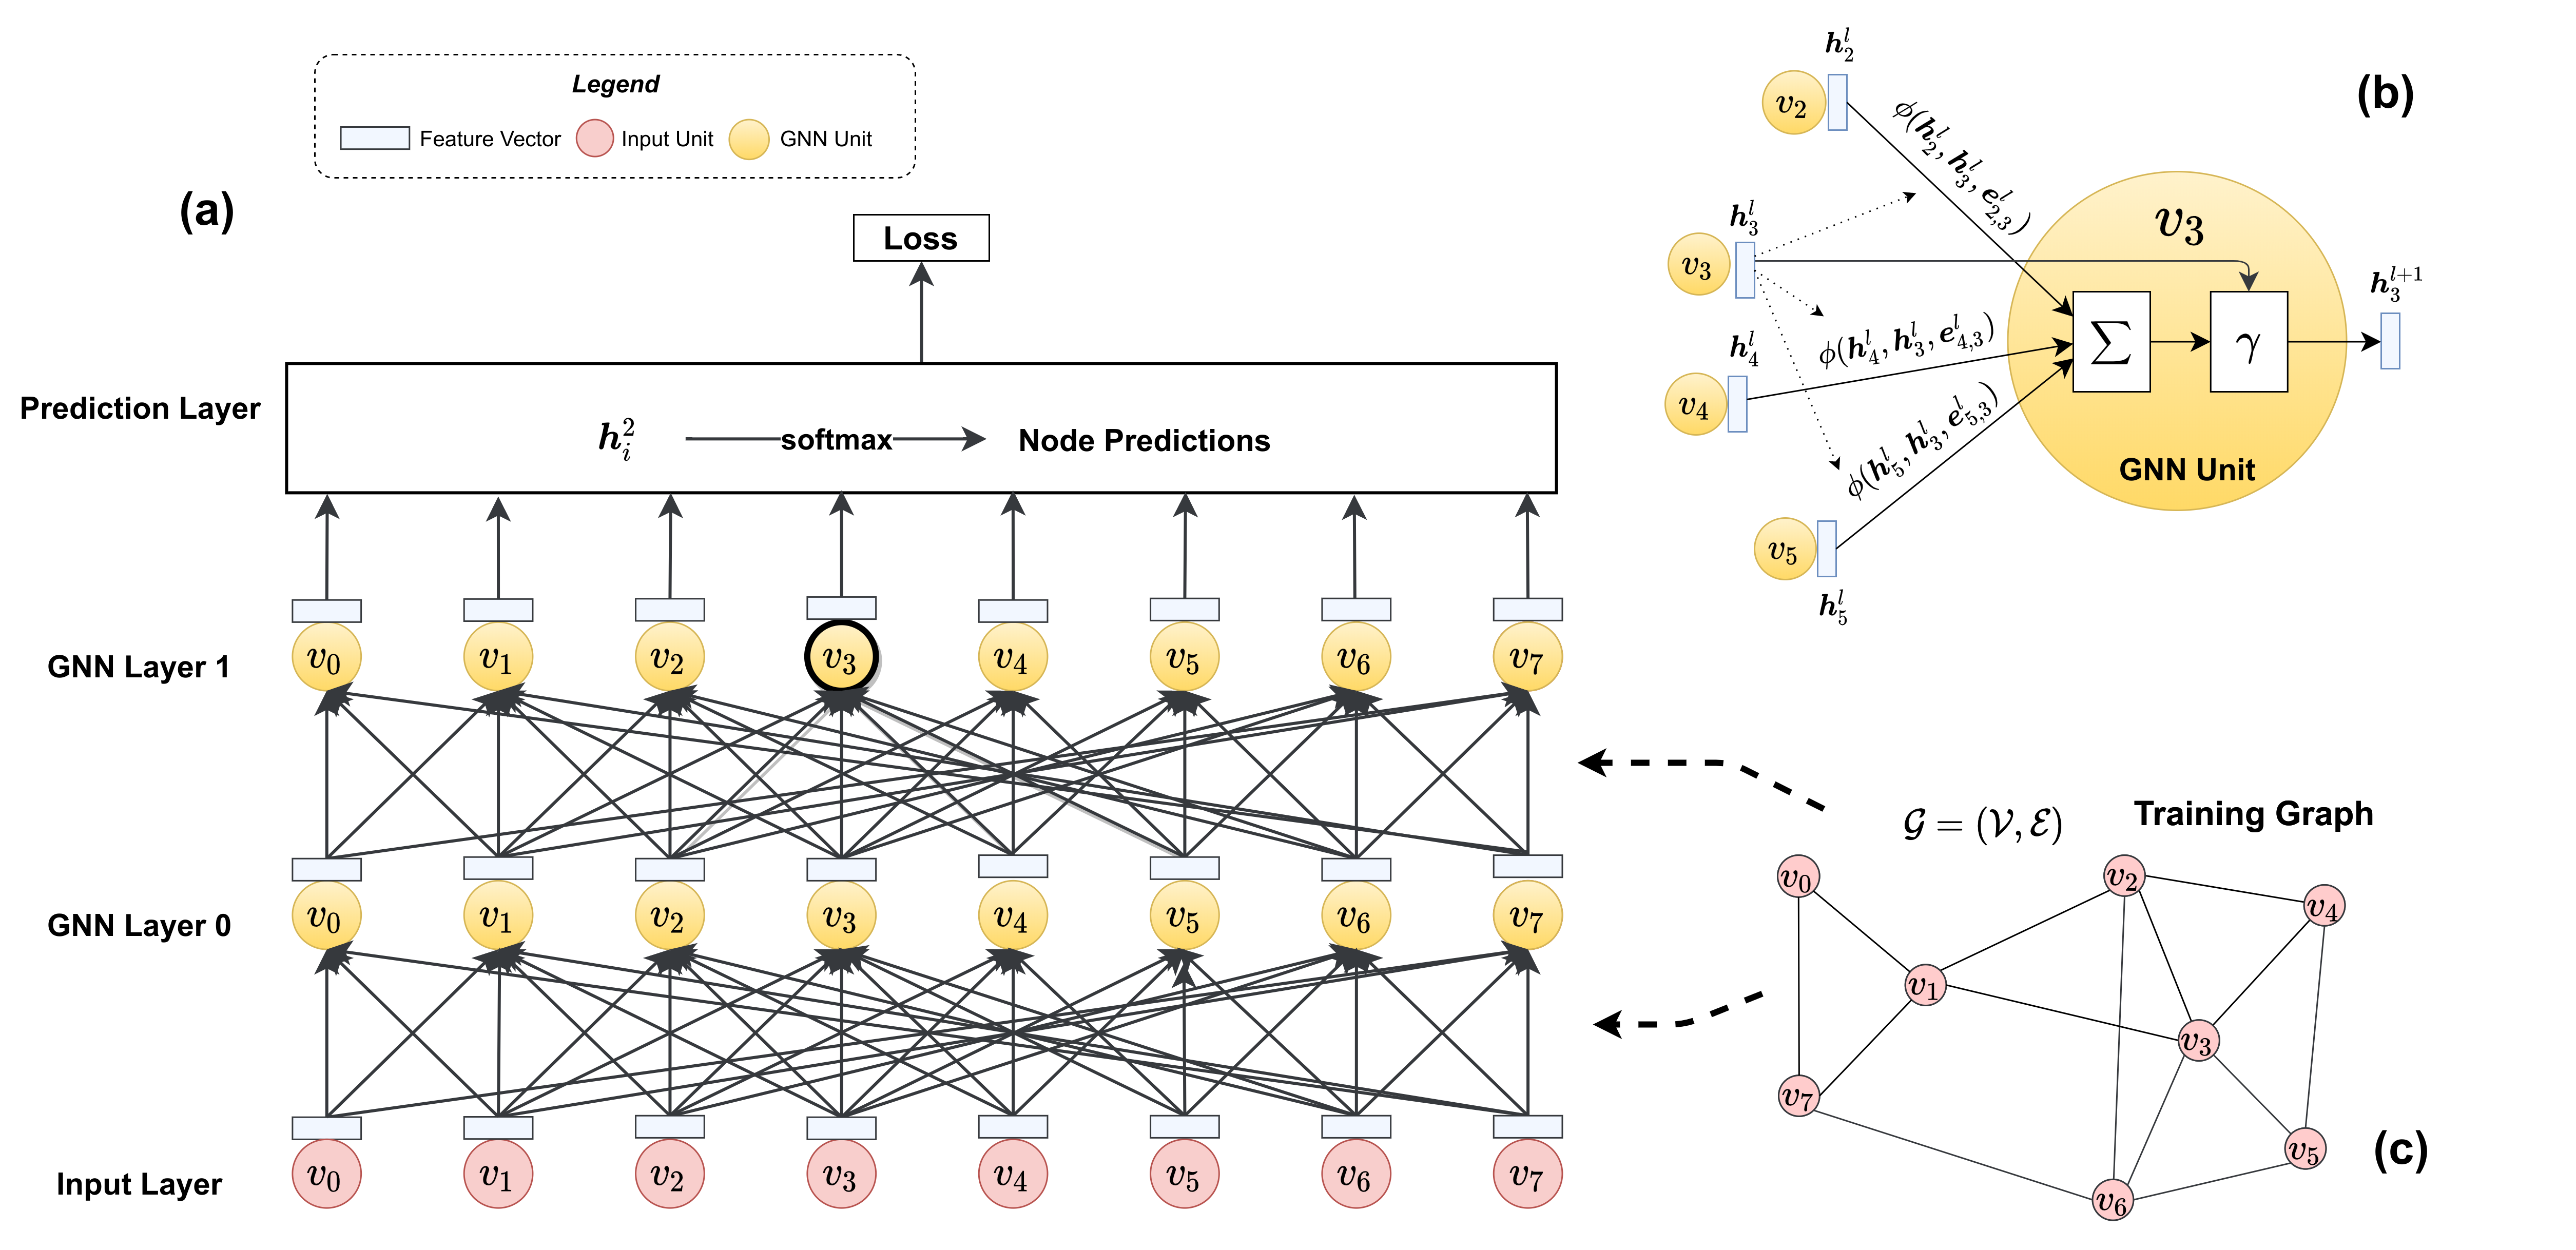
\includegraphics[width=0.95\columnwidth]{figs/illustration/GNN_common_architecture.png}
	\caption{Structure of a typical graph neural network. (a) Demo GNN; (b) GNN unit; (c) Demo graph. The target application is the node classification. The demo GNN has two GNN layers.}
	\label{fig:general_structure_of_gnn}
\end{figure}

A GNN receives a graph $\mathcal{G}$ as the input.
Every vertex $v_i$ in $\mathcal{G}$ is attached with a feature vector $\boldsymbol{x}_i$ to describe the properties of the vertex.
The input layer of a GNN receives feature vectors from all vertices and passes them to GNN layers.

A GNN layer consists of $n$ GNN units, where $n$ is the number of vertices in $\mathcal{G}$.
Each GNN unit correspond to a vertex in $\mathcal{G}$.
In the first GNN layer (Layer 0), the GNN unit of the vertex $v_i$ collects input feature vectors of the vertices $\boldsymbol{x}_j$ that are adjacent to $v_i$ in $\mathcal{G}$ (i.e., $j \in \mathcal{N}(v_i)$) from the input layer.
In other words, the connection between the input layer and the first GNN layer is determined by the topology of $\mathcal{G}$.
In the traditional neural networks, the neural units of neighboring layers are fully connected.
In GNNs, two GNN units are connected only if they have an edge between them in $\mathcal{G}$, which is usually \emph{sparse}.
After aggregating input feature vectors and applying non-linear transformation, the GNN unit outputs a hidden feature vector $\boldsymbol{h}^1_i$ for $v_i$.

In the next GNN layer (Layer 1), the GNN unit of $v_i$ collects the hidden feature vectors $\boldsymbol{h}^1_j$ of $v_i$'s neighbors (i.e., $j \in \mathcal{N}(v_i)$) from the \emph{previous} GNN layer.
The connection between neighboring GNN layers are also determined by $\mathcal{E}$ of $\mathcal{G}$.
Based on the collected hidden vectors, the GNN unit in Layer 1 outputs a new hidden feature vector $\boldsymbol{h}^2_i$ for $v_i$.
A GNN allows to stack more GNN layers to support deeper graph analysis.
%In \figurename~\ref{fig:general_structure_of_gnn}, we shows a GNN with two layers.

Assume there are $L$ GNN layers.
The last GNN layer (Layer $L-1$) outputs a hidden feature vector $\boldsymbol{h}^{L}_i$ for every vertex $v_i$.
As an embedding vector, $\boldsymbol{h}^L_i$ encodoes the knowledge learned from the input layer and all the previous GNN layers.
Finally, $\boldsymbol{h}^L_i$ is affected by $v_i$ and all the vertices in the $L$-hop neighborhood of $v_i$.
Analyzing with deeper GNNs means analyzing each vertices with a wider scope.

The hidden feature vectors $\boldsymbol{h}^L_i$ of the last GNN layer are fed to the prediction layer to generate the output of the whole GNN.
The prediction layer is a standard nerual network.
The structure of the prediction layer depends on the prediction task of the GNN.
Take the node classification task as the example, as shown in \figurename~\ref{fig:general_structure_of_gnn}.
The node classification predicts a label for every vertex in $\mathcal{G}$.
In this case, the prediction layer can be a simple softmax layer with $\boldsymbol{h}^L_i$ as the input and a vector of probabilities as the output.
If the prediction task is edge prediction, the hidden feature vectors of two vertices are concatenated and fed into a softmax layer.
If we need to predict a label for the whole graph, a pooling (max/mean/...) layer is added to generate an embedding vector for the whole graph and the embedding vector is used to produce the final prediction.

Supporting end-to-end training is a prominent advantage of GNN, compared with other graph-based machine learning methods.
We can calculate the gradients of the loss function on the model parameters from the prediction layer directly.
With the help of the back proporgation technique, the gradient is propogated from the prediction layer back to the previous GNN layers layer by layer.
The model parameters are updated with a gradient descent optimizer like Adam.
Except for the input feature vector, there is no need to conduct handworked feature extraction.
In a fully parameterized way, the GNN automatically extracts an embedding vector for each vertex from its $L$-hop neighborhood.
The parameters are tuned according to the specific prediction task, leading to high prediction accuracy.

\subsection{GNN Unit and Message-passing Model}
